\def\duedate{\today}
\def\HWnum{4}
\documentclass[10pt,a4paper]{book}

% custom section formatting
\usepackage{titlesec}
\titleformat{\chapter}[display]
{\normalfont\Large\filcenter\sffamily}
{\titlerule[1pt]%
\vspace{1pt}%
\titlerule
\vspace{1pc}%
\LARGE\MakeUppercase{\chaptertitlename} \thechapter}
{1pc}
{\titlerule
\vspace{1pc}%
\Huge}

% appendix handling
\usepackage[toc,page]{appendix}
    
% encoding for file and font
\usepackage[utf8]{inputenc}
\usepackage[T1]{fontenc}

% math formatting/tools
\usepackage{amsmath}
\usepackage{amssymb}
\usepackage{mathtools}
\usepackage[arrowdel]{physics}
\usepackage{dsfont}

\newcommand{\R}{\mathbb{R}}
\newcommand{\Z}{\mathbb{Z}}
\newcommand{\N}{\mathbb{N}}
\newcommand{\Q}{\mathbb{Q}}
\newcommand{\C}{\mathbb{C}}

% unit formatting
\usepackage{siunitx}
\AtBeginDocument{\RenewCommandCopy\qty\SI}

% figure formatting/tools
\usepackage{graphicx}
\usepackage{float}
\usepackage{subcaption}
\usepackage{multirow}
\usepackage{import}
\usepackage{pdfpages}
\usepackage{transparent}
\usepackage{currfile}

\NewDocumentCommand\incfig{O{1} m}{
    \def\svgwidth{#1\textwidth}
    \import{./Figures/\currfiledir}{#2.pdf_tex}
}

\newcommand{\bef}{\begin{figure}[h!tb]\centering}
\newcommand{\eef}{\end{figure}}

\newcommand{\bet}{\begin{table}[h!tb]\centering}
\newcommand{\eet}{\end{table}}

% hyperlink references 
\usepackage{hyperref}
\hypersetup{
    colorlinks=true,
    linkcolor=blue,
    filecolor=magenta,
    urlcolor=cyan,
    pdftitle={Physics 1 Notes},
    pdfauthor={Richard Whitehill},
    pdfpagemode=FullScreen
}
\urlstyle{same}

\newcommand{\eref}[1]{Eq.~(\ref{eq:#1})}
\newcommand{\erefs}[2]{Eqs.~(\ref{eq:#1})--(\ref{eq:#2})}

\newcommand{\fref}[1]{Fig.~(\ref{fig:#1})}
\newcommand{\frefs}[2]{Fig.~(\ref{fig:#1})--(\ref{fig:#2})}

\newcommand{\aref}[1]{Appendix~(\ref{app:#1})}
\newcommand{\sref}[1]{Section~(\ref{sec:#1})}
\newcommand{\srefs}[2]{Sections~(\ref{sec:#1})-(\ref{sec:#2})}

\newcommand{\tref}[1]{Table~(\ref{tab:#1})}
\newcommand{\trefs}[2]{Table~(\ref{tab:#1})--(\ref{tab:#2})}

% tcolorbox formatting/definitions
\usepackage[most]{tcolorbox}
\usepackage{xcolor}
\usepackage{xifthen}
\usepackage{parskip}

\definecolor{peach}{rgb}{1.0,0.8,0.64}

\DeclareTColorBox[auto counter, number within=chapter]{defbox}{O{}}{
    enhanced,
    boxrule=0pt,
    frame hidden,
    borderline west={4pt}{0pt}{green!50!black},
    colback=green!5,
    before upper=\textbf{Definition \thetcbcounter \ifthenelse{\isempty{#1}}{}{: #1} \\ },
    sharp corners
}

\newcommand*{\eqbox}{\tcboxmath[
    enhanced,
    colback=black!10!white,
    colframe=black,
    sharp corners,
    size=fbox,
    boxsep=8pt,
    boxrule=1pt
]}

\newtcolorbox[auto counter, number within=chapter]{exbox}{
    parbox=false,
    breakable,
    enhanced,
    sharp corners,
    boxrule=1pt,
    colback=white,
    colframe=black,
    before upper= \textbf{Example \thetcbcounter:}\,,
    before lower= \textbf{Solution:}\,,
    segmentation hidden
}

\newtcolorbox{resbox}{
    enhanced,
    colback=black!10!white,
    colframe=black,
    boxrule=1pt,
    boxsep=0pt,
    top=2pt,
    ams nodisplayskip,
    sharp corners
}


\begin{document}

\prob{1}{

    What are the lines of constant $u(x,y)$ and $v(x,y)$ for the function $f(z) = u(x,y) + iv(x,y) = \ln{z}$?

}

\sol{

We can write
\begin{eqnarray}
    \ln{z} = \ln{r} + i \theta
,\end{eqnarray}
where we restrict $\theta \in [0,2\pi)$ such that $\ln{z}$ is single-valued.
Thus,
\begin{align}
    u(x,y) &= \ln{r} \\
    v(x,y) &= \theta
,\end{align}
where $r = \sqrt{x^2 + y^2}$ and $\tan{\theta} = y/x$.
Hence, lines of constant $u$ are circles of radius $r$ in the complex plane while lines of constant $v$ are lines that make angle $\theta$ relative to the real axis (as shown in \fref{prob1}).

\begin{figure}[h!]
   \centering
   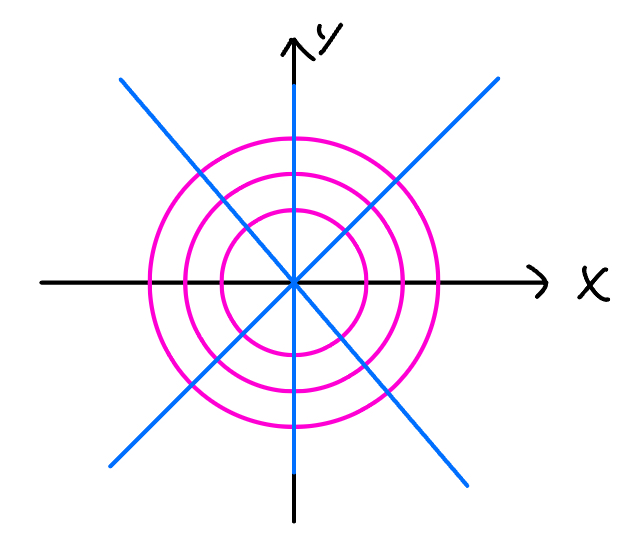
\includegraphics[width=0.3\textwidth]{prob1.jpeg}
   \caption{Sketch of lines of constant $u$ (magenta) and $v$ (blue).}
   \label{fig:prob1}
\end{figure}

}


\prob{2}{

Calculate the integral
\begin{eqnarray}
    I(\alpha) = \oint_{|z|=1} z^{\alpha} \dd{z}
\end{eqnarray}
along the circle of radius $|z|=1$, where $\alpha \in \reals$.

}

\sol{

This integral is computed as follows:
\begin{eqnarray}
    \eqbox{
    \begin{aligned}
        I(\alpha) &= \int_{0}^{2 \pi} e^{i \alpha \theta} (i e^{i \theta}) \dd{\theta} = \int_{0}^{2 \pi} e^{i (\alpha + 1) \theta} \dd{\theta} \\
          &= \frac{1}{i (\alpha + 1)} \Big[ e^{i (\alpha + 1) 2 \pi} - 1 \Big] = \frac{e^{2 \pi i \alpha} - 1}{i (\alpha + 1)}
    .\end{aligned}
}
\end{eqnarray}
Notice that, as found in class, if $\alpha = 0, 1, \pm 2, \pm 3, \ldots$, the result is identically zero.
If $\alpha = -1$, then $I(\alpha) = 2 \pi i$.

Now, let us restrict our attention to non-integer $\alpha$.
Upon first sight, it may seem that $I(\alpha) \equiv 0$ for such $\alpha$, but upon closer inspection, one notices that the function $z^{\alpha}$ is multi-valued (finitely multi-valued for rational $\alpha$ and infinitely multi-valued for irrational $\alpha$).
Thus, $z^{\alpha}$ is not analytic everywhere inside $C$ for $\alpha \not\in \integers$, and we must enforce some branch cut when defining $z^{\alpha}$ such that it is single-valued.

Actually, $I(\alpha)$ takes on different values for different choices of branch cut.
For example, in the computation above, we implicitly chose the branch cut along the real, positive axis.
If we chose, however, the branch cut along the real, negative axis such that $\theta \in [-\pi,\pi)$, then
\begin{eqnarray}
    I(\alpha) = -\frac{e^{i \pi \alpha} - e^{-i \pi \alpha}}{i (\alpha + 1)} = -\frac{2}{\alpha + 1} \sin{ \pi \alpha }
.\end{eqnarray}
The integrations choosing different branch cuts are different by a phase.


}

\prob{3}{

Calculate the integral
\begin{eqnarray}
    I = \oint_{C} \frac{z + 1}{z^2 + 4} \dd{z} ~ {\rm if:}
\end{eqnarray}
(a) The point $2i$ is inside the contour $C$, and the point $-2i$ is outside the contour $C$.
(b) The point $-2i$ is inside the contour $C$, and the point $2i$ is outside the contour $C$.
(c) Both points $2i$ and $-2i$ are inside the contour $C$.

}

\sol{

Observe that we can write
\begin{eqnarray}
   f(z) = \frac{z + 1}{z^2 + 4} = \frac{z + 1}{(z - 2i)(z + 2i)}
,\end{eqnarray}
which has poles at $\pm 2i$, and according to Cauchy's integral theorem

(a) if $C$ encloses the pole at $2 i$ but not that at $- 2 i$, then
\begin{eqnarray}
   \eqbox{
       I = 2 \pi i \Big[ \frac{z + 1}{z + 2i} \Big]_{z = 2i} = \frac{\pi}{2}(1 + 2i)
   } 
.\end{eqnarray}

(b) On the other hand, if $C$ encloses the pole at $-2 i$ but not that at $2i$, then
\begin{eqnarray}
   \eqbox{
       I = 2 \pi i \Big[ \frac{z + 1}{z - 2i} \Big]_{z = -2i} = -\frac{\pi}{2}(1 - 2i)
   } 
.\end{eqnarray}

(c) Now, if $C$ encloses both poles, the result is just the sum of the previous two:
\begin{eqnarray}
    \eqbox{
        I = \frac{\pi}{2} \Big[ (1 + 2i) - (1 - 2i) \Big] = 2 \pi i
    }
.\end{eqnarray}
This fact can be seen easily.
In our derivation of Cauchy's integral theorem, we only worried about a function with one simple pole, which we handled by ``removing'' it from the integration region.
For a function with $n$ poles enclosed by $C$, we just repeat the argument at each pole, ``removing'' each of them individually, which gives us
\begin{eqnarray}
    \sum_{k=1}^{n} \phi_{k}(z_{k}) = \frac{1}{2 \pi i} \int_{C} f(z) \dd{z}
,\end{eqnarray}
where $\phi_{k}(z) = (z - z_{k})f(z)$.
Alternatively, and more concretely, we could handle this particular case by writing $C = C_+ + C_-$, where $C_{\pm}$ encloses only the pole at $z = \pm 2i$.

\begin{figure}[h!]
   \centering
   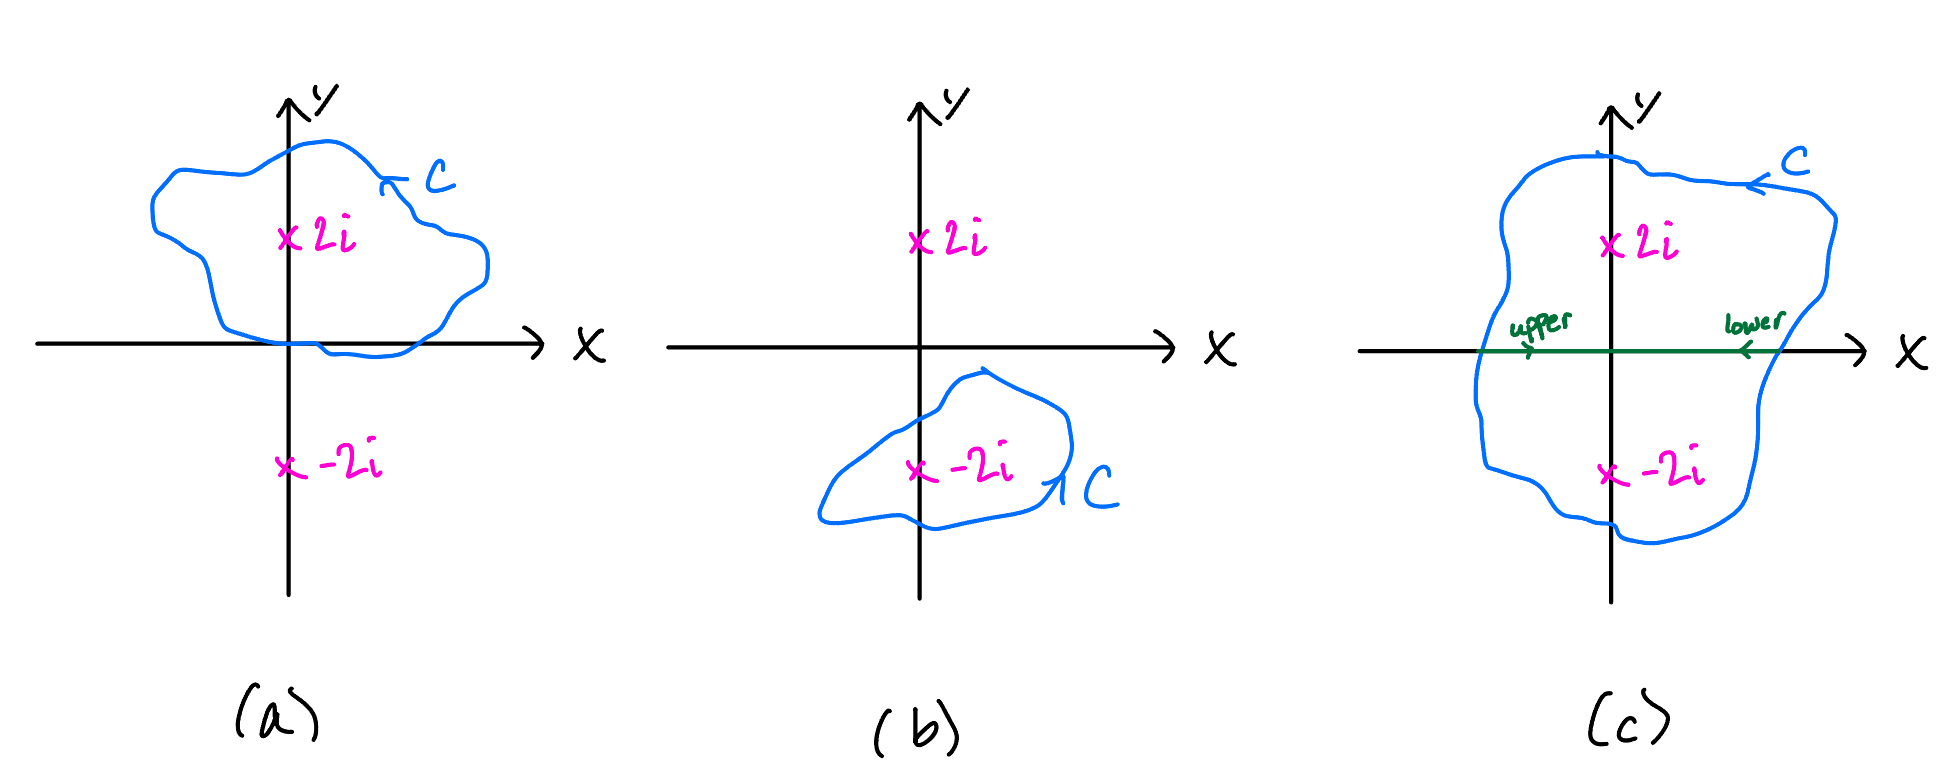
\includegraphics[width=\textwidth]{prob3.jpeg}
   \caption{Sketch of contours which enclose \textbf{(a)} $z = 2i$, \textbf{(b)} $z = -2i$, and \textbf{(c)} $z = \pm 2i$. Also note that the green line along the real axis in (c) gives an idea for how to ``break'' $C$ into separate paths $C_{\pm}$, which individually enclose $z = \pm 2i$ and whose contributions cancel when the contour integrals of $C_{\pm}$ are summed.}
   \label{prob3}
\end{figure}

}

\prob{4}{

The function defined by the series
\begin{eqnarray}
    I_{4}(z) = \frac{1}{1 + z^2} = 1 - z^2 + z^{4} - z^{6} + \ldots = \sum_{n=0}^{\infty} (-1)^{n} z^{2n}
\end{eqnarray}
is convergent at $|z| < 1$.
Find the convergent series which analytically continues this function into the region $|z| > 1$.

}

\sol{

Notice
\begin{eqnarray}
    \eqbox{
    \begin{aligned}
        I_4(z) &= \frac{1}{z^2} \frac{1}{1 - (-z^{-2})} = \frac{1}{z^2} \Big[ 1 - \frac{1}{z^2} + \frac{1}{z^{4}} - \frac{1}{z^{6}} + \ldots \Big] \\
               &= \frac{1}{z^2} - \frac{1}{z^{4}} + \frac{1}{z^{6}} - \frac{1}{z^{8}} + \ldots
    ,\end{aligned}
}
\end{eqnarray}
which is valid for $|1/z^2| > 1$ or $|z| > 1$.

}

%\newpage

\prob{5}{

Expand the following function in the Laurent series in the neighborhood of $z = \infty$:
\begin{eqnarray}
    I_{5}(z) = \ln{\frac{z^2 - a^2}{z^2 - b^2}}
.\end{eqnarray}

}

\sol{

Let us make the spatial inversion $t = 1/z$\footnote{This allows us to expand $I_{5}(1/t)$ about $t=0$, which is by construction an expansion of $z$ in the neighborhood of $\infty$.}, which allows us to write
\begin{eqnarray}
    I_{5}(z) = \ln( \frac{1 - t^2a^2}{1 - t^2b^2} ) = \ln(1 - t^2a^2) - \ln(1 - t^2b^2)
,\end{eqnarray}
and since $\ln(1 + x) = x - x^2/2 + x^3/3 - x^{4}/4 \ldots$, we have
\begin{eqnarray}
    \eqbox{
    \begin{aligned}
        I_{5}(z) &= \sum_{n=1}^{\infty} \frac{(-1)^{n+1}}{n} (-t^2 a^2)^{n} - \sum_{n=1}^{\infty} \frac{(-1)^{n+1}}{n} (-t^2 b^2)^{n} \\
                 &= \sum_{n=1}^{\infty} \frac{1}{n} \frac{b^{2n} - a^{2n}}{z^{2n}} \\
                 &= \frac{b^2 - a^2}{z^2} + \frac{b^{4} - a^{4}}{z^{4}} + \frac{b^{6} - a^{6}}{z^{6}} + \ldots
    ,\end{aligned}
}
\end{eqnarray}
where in the second-to-last line, we have replaced $t$ with $z$ to make the expansion in $z$ explicit.

}

\prob{6}{

Expand the following function in the Laurent series at $z = 0$:
\begin{eqnarray}
    I_{6}(z) = z^3 \exp(-\frac{1}{z^2})
.\end{eqnarray}

}

\sol{

This can be done as follows:
\begin{eqnarray}
    \eqbox{
    \begin{aligned}
        I_6(z) &= z^3 \sum_{n=0}^{\infty} \frac{1}{n!} \Big( -\frac{1}{z^2} \Big)^{n} = \sum_{n=0}^{\infty} \frac{(-1)^{n}}{n! \, z^{2n - 3}} \\
               &= z^3 - z + \frac{1}{2 z} - \frac{1}{6 z^3} + \ldots
    .\end{aligned}
}
\end{eqnarray}


}


\end{document}
